\documentclass{article}
\usepackage{fancyhdr}
\usepackage{epigraph}
\usepackage{pdfpages}

\pagestyle{fancy}
\fancyhf{}
\lhead{Math 110}
\chead{Project 2}
\rhead{Due: March 29, 2019}
\cfoot{\thepage}


\begin{document}
Salaries can vary greatly depending on your degree, type of employment, and location; cost of living can also largely vary between different locations in the world. The goal of this project is to compare salaries and costs of living in different cities (within the US). You will complete this project in your assigned groups. Each group will do a summary presentation for the class; your group will be graded based on the summary presentation; a completed project essay (1 per group) will be submitted as well.

\section*{Part 1: Gathering Data}
\begin{enumerate}
	\item Each member of your group should decide what sort of career they want to have as well as a list of three cities in which they may be interested in living.
	\item Using the Occupational Outlook Handbook {\tt https://www.bls.gov/ooh/}, each group member should identify what the national median and average salaries are for your chosen occupation.  Also, look up what each person could expect to earn in your selected cities.
	\item Tax rates vary according to income levels; for purposes of this project, make it easy and assume the total withheld for all taxes is 18\% of the gross salary. Remember that ‘disposable income’ is the amount that remains after taxes. Determine each group member’s ‘disposable income’ based on the median salary in each city.
	\item Using the budgeting guidelines found at {\tt https://www.nomoredebts.org/budgeting-guidelines}, construct a budget for the disposable income which you would realize in each city.
	\item Each group member should investigate the actual cost of living in each of their selected cities as well as their home town.  Use the cost of living calculator at {\tt https://www.payscale.com/cost-of-living-calculator} to start this investigation.  You may also want to seek out additional resources.  What you will try to do is work out what your life would be like in each city.  Where is the optimal place for you to practice your chosen profession?
\end{enumerate}
\section*{Part 2: Essay}
Construct a 1500 - 2500 word essay using your groups data. The formatting and citation
requirements for this essay are identical to what we had in the first project.  Your essay should include the following information:
\begin{itemize}
	\item Salary projections for each group member.
	\item Comparison of the national median and the median in your three selected cities.
	\item Comparison of the budgets you would have in the cities you have chosen based on OOHB data.
	\item Comparison of the cost of living in each of the cities, with special attention being paid to how adequate your income would be for living in each city.  Are any too expensive for you?
	\item A discussion of how your region and profession fit together.  Are there cities that universally pay more, or is it dependent on both variables?
	\item At least three cited sources other than the ones mentioned in this writing prompt.
\end{itemize}

Remember, you will be graded as a group.  You will submit one essay that brings together all of your collected information.  The essay will comprise 80\% of your project grade.

\section*{Part 3: Presentation}
Construct a presentation (in power point or some other software) which summarizes the information from your essay.  Your presentation should be 5-10 minutes in length.  Points will be deducted for presentations that are under or over time.  The rubric by which the presentations are graded is on the next page.  The presentation score will comprise 20\% of your grade.  You are also required to be present for all presentations.  If you are absent during a presentation day, you will receive a grade of zero for this project.

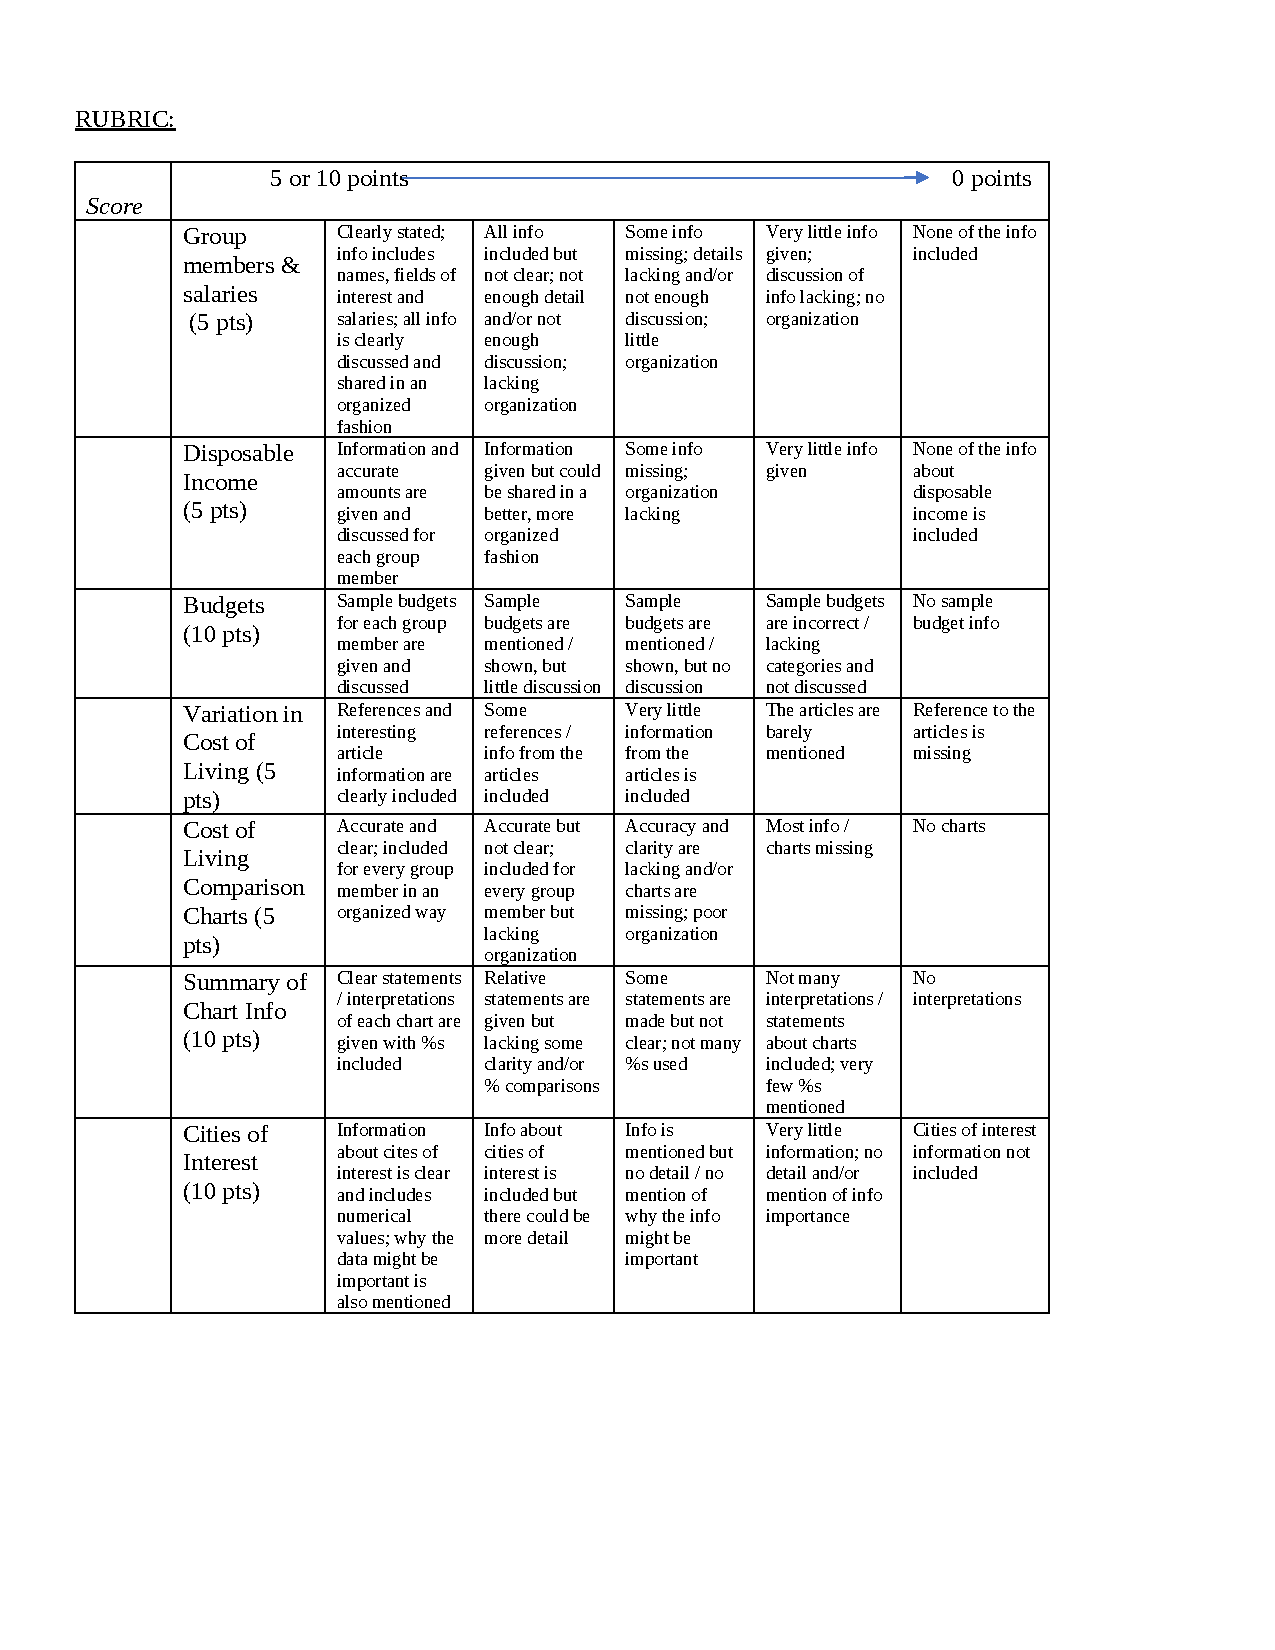
\includepdf[angle=90]{presentation-rubric}
\end{document}